\chapter{从熵与能量得到温度}

\lectureoverview{温度最初表现为将人的温度计单位换算为微观能量单位。在完成从热力学熵到无量纲统计熵的相应换算之后，我们用一族单参数概率分布描述平衡态。导数\(dE/dS\)于是定义了温度，而前两条定律说明了为什么温度差决定能量流动的方向。}

\section{换算因子与人的单位}

物理学中的许多常数都是换算因子。光速把距离换算为时间：
\begin{equation}
 t=\frac{x}{c}.
\end{equation}
如果距离和时间用相容的单位测量，就可以令\(c=1\)。没有任何物理效应消失；只是把两类测量放到了同一个共同的标度上。

玻尔兹曼常数具有同样的性质。它把在人的尺度温度计上读出的温度换算为能量。\emph{人的尺度}这个形容词很重要。选择这样的单位，是因为宏观仪器能够产生并分辨它们，而不是因为微观动力学特别挑中了它们。

摄氏度是通过把标准压强下水的凝固点与沸点之间的间隔分成一百份来确定的。开尔文使用大小相同的度，但把零点放在绝对零度处。选择不同的物质、不同的间隔或华氏度，会改变数值，但不会改变物理。

\begin{classroomqa}
\audiencequestion{华氏温标已经是十七世纪的构造了吗？}
\lecturerresponse{这里不需要精确的日期。要点在于，所有这类温标都是围绕人们能够制备和测量的温度设计的。它们的度的大小是约定的，而不是微观的。
\lecturetimestamp{00:01:34--00:01:50}}
\end{classroomqa}

在这些温标被创造出来的时代，实验还无法获得热的分子起源。一度的变化可以用宏观温度计观察到，而一个分子的能量却无法测量。因此，在任何人知道温度从根本上是一个能量标度之前，发明一个温度单位是很自然的。

\section{为什么温度具有能量的单位}

考虑稀薄单原子气体。稀薄意味着就目前的目的而言，分子之间的相互作用能可以忽略。在热平衡中，能量均分给每个平动二次自由度分配\(T_{\mathrm K}/2\)乘以玻尔兹曼常数。在三个空间维度中，
\begin{equation}
 \left\langle E_{\mathrm{kin}}\right\rangle
 =\frac{3}{2}k_{\mathrm B}T_{\mathrm K}.
 \label{eq:sm2-equipartition-kelvin}
\end{equation}
因子三计入沿\(x\)、\(y\)和\(z\)方向的运动。因子二分之一来自二次动能。

这个关系并非某种分子所特有。在处于平衡的氦与氧的混合物中，每个自由平动的粒子都具有相同的平均质心动能，尽管较重的粒子运动得更慢。由于
\begin{equation}
 E_{\mathrm{kin}}=\frac{1}{2}mv^2,
\end{equation}
相同的特征能量意味着\(v\propto m^{-1/2}\)。

同样的想法可以推到一个刻意极端的例子。把一个保龄球悬浮在流体中，让整个系统达到平衡。它的布朗平动自由度由与分子相同的能量标度支配。球的速度小得不可思议，因为它的质量大得不可思议，但温度比较的是能量标度，而不是速率。

在室温下，\(T_{\mathrm K}\)约为\(300\,\mathrm K\)，而一个微观自由度的能量以焦耳计则极小。因此换算因子极小：
\begin{equation}
 k_{\mathrm B}\simeq 1.38\times10^{-23}\,
 \mathrm{J\,K^{-1}}.
 \label{eq:sm2-boltzmann-value}
\end{equation}
它的尺度与阿伏伽德罗数之间的关系并非巧合，而是相互关联的：
\begin{equation}
 R=N_{\mathrm A}k_{\mathrm B}.
\end{equation}
气体常数\(R\)描述一摩尔，而\(k_{\mathrm B}\)描述每个微观组分相应的标度。

基本公式中反复出现组合
\(k_{\mathrm B}T_{\mathrm K}\)。因此更简洁的做法是定义
\begin{equation}
 T\equiv k_{\mathrm B}T_{\mathrm K}.
 \label{eq:sm2-energy-temperature}
\end{equation}
从现在起，\(T\)本身就具有能量的单位，而
\eqref{eq:sm2-equipartition-kelvin}变为
\begin{equation}
 \left\langle E_{\mathrm{kin}}\right\rangle=\frac{3}{2}T.
 \label{eq:sm2-equipartition-natural}
\end{equation}
如果能量以焦耳测量，温度就以焦耳测量。如果能量以电子伏测量，温度就以电子伏测量。并不存在一种自然界的新单位叫作温度单位。

\section{熵的两种约定}

同样的换算也出现在熵这一侧。宏观热力学是从对热机的分析中发展出来的。卡诺提供了决定性的热机推理；克劳修斯后来引入了热力学熵和符号\(S\)。在本书使用的记号中，把这个宏观量称为\(S_{\mathrm C}\)。它的单位是能量除以温度计温度，例如焦耳每开尔文。

统计熵是无量纲的。对于离散分布，
\begin{equation}
 S=-\sum_i p_i\log p_i.
 \label{eq:sm2-statistical-entropy}
\end{equation}
采用自然对数时，一个公平的二元备择具有熵 \(\log2\)；采用以2为底的对数时，同样的量称为一比特。这两种熵约定之间的关系为
\begin{equation}
 S=\frac{S_{\mathrm C}}{k_{\mathrm B}},
 \qquad
 S_{\mathrm C}=k_{\mathrm B}S.
 \label{eq:sm2-entropy-conversion}
\end{equation}
一个在 \(\mathrm{J\,K^{-1}}\) 中适中的宏观值对应于一个巨大的无量纲熵，因为它计数的信息分布在数量极其庞大的微观组分之中。

方程 \eqref{eq:sm2-energy-temperature} 和
\eqref{eq:sm2-entropy-conversion} 确立了贯穿全书的约定：
\[
 [T]=[\text{energy}],
 \qquad
 [S]=1.
\]
玻尔兹曼常数现在可以从工作公式中消失。它总是可以通过将 \(T\) 替换为 \(k_{\mathrm B}T_{\mathrm K}\) 并将 \(S\) 替换为 \(S_{\mathrm C}/k_{\mathrm B}\) 来恢复。

\begin{classroomqa}
\audiencequestion{除了因子 \(3/2\) 之外，新温度难道不就是以焦耳计量的能量吗？}
\lecturerresponse{是的，如果焦耳是所选择的能量单位。焦耳是MKS单位 \(\mathrm{kg\,m^2\,s^{-2}}\)。人们也可以改用电子伏特或任何其他能量单位；那么温度就必须用同一单位来表示。因子 \(3/2\) 属于理想气体这个例子，而不属于温度的定义。
\lecturetimestamp{00:15:49--00:16:45}}
\end{classroomqa}

\begin{classroomqa}
\audiencequestion{如果黑板上指定了开尔文，那么 \(k_{\mathrm B}\) 不就是一个确定的常数吗？}
\lecturerresponse{在温度和能量单位都被指定之后，它是确定的。把开尔文改为华氏度，或者把焦耳改为电子伏特，它的数值就会改变。这种对单位的依赖性正是换算因子的行为。
\lecturetimestamp{00:16:46--00:18:33}}
\end{classroomqa}

\begin{classroomqa}
\audiencequestion{玻尔兹曼常数的数值是由实验确定的吗？}
\lecturerresponse{是的。历史上，它的求值需要关于原子及其数密度的微观信息。玻尔兹曼在这些量被精确知道之前就理解了分子能量与温度之间的关系，正如牛顿在引力常数被精确测量之前就知道它的作用一样。
\lecturetimestamp{00:18:46--00:20:00}}
\end{classroomqa}

\section{平衡是一种统计状态}

单位换算仍然没有定义温度。触摸热的东西会给出有用的生物学直觉，但温度是由能量和熵构建出来的导出物理量。

想象一个系统与一个宏观条件固定的大环境接触。能量可以在它们之间传递。如果系统最初能量过多，它平均而言会失去能量；如果能量过少，它平均而言会获得能量。在热平衡中，微观交换仍在继续，但两个方向上都没有净的平均流动。

令 \(i\) 标记系统的一个精确微观状态，并令 \(E_i\) 为该状态的能量。平衡并不意味着系统冻结在一个状态中。它与环境的相互作用不断改变微观状态，因此我们为每一种可能性赋予一个概率 \(P_i\)。基本关系是
\begin{align}
 \sum_i P_i &=1,
 \label{eq:sm2-normalization}\\
 \sum_i P_iE_i &=\overline E,
 \label{eq:sm2-mean-energy}\\
 S&=-\sum_iP_i\log P_i.
 \label{eq:sm2-equilibrium-entropy}
\end{align}
\(\overline E\) 上的横线强调子系统的能量在涨落。一次测量可能给出一个值，下一次测量可能给出另一个值；重复测量会稳定到其平均值为 \eqref{eq:sm2-mean-energy} 的分布。

\begin{figure}[t]
\centering
\includegraphics[width=0.82\textwidth]{lecture_02_figure_02.png}
\caption{黑板上的归一化和平均能量：
\(\sum_iP(i)=1\) 和 \(\sum_iP(i)E(i)=\langle E\rangle\)。}
\lectureframe{00:24:10}
\end{figure}

\section{以平均能量标记的族}

平衡分布强烈依赖于平均能量。把一壶水放在炉子上，\(\overline E\) 上升；把它放在雪中，\(\overline E\) 下降。概率随之改变。因此，平衡不应被视为一个分布，而应被视为一个单参数族：
\begin{equation}
 P_i(\overline E).
 \label{eq:sm2-family}
\end{equation}
每一个成员都满足
\begin{align}
 \sum_iP_i(\overline E)&=1,
 \label{eq:sm2-family-normalization}\\
 \sum_iP_i(\overline E)E_i&=\overline E.
 \label{eq:sm2-family-mean}
\end{align}

\begin{figure}[t]
\centering
\includegraphics[width=0.88\textwidth]{lecture_02_figure_03.png}
\caption{向 \(P(i,\overline E)\) 的过渡。在引入分布族的同时，先前的归一化、平均能量和熵方程仍然可见。}
\lectureframe{00:26:29}
\end{figure}

对于示意图，按 \(E_i\) 递增的顺序排列状态。横轴于是既可以读作指标 \(i\)，也可以读作相应的能量。更高的平均能量将概率权重移向更靠右的状态。每条曲线都必须保持单位总面积。

\begin{figure}[t]
\centering
\includegraphics[width=0.88\textwidth]{lecture_02_figure_04.png}
\caption{若干示意性分布 \(P(i,\overline E)\)。权重更靠右的曲线具有更大的平均能量，而每条曲线都保持归一化。}
\lectureframe{00:28:40}
\end{figure}

\begin{figure}[t]
\centering
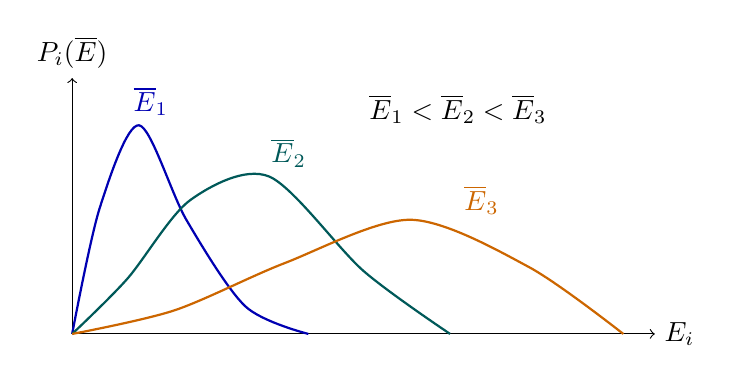
\begin{tikzpicture}[x=1cm,y=1cm]
\draw[->] (0,0) -- (7.4,0) node[right] {$E_i$};
\draw[->] (0,0) -- (0,3.25) node[above] {$P_i(\overline E)$};
\draw[thick,blue!70!black]
  plot[smooth] coordinates {(0,0) (0.35,1.6) (0.85,2.65) (1.45,1.45)
  (2.2,0.35) (3.0,0)};
\draw[thick,teal!70!black]
  plot[smooth] coordinates {(0,0) (0.7,0.7) (1.5,1.7) (2.5,2.0)
  (3.7,0.8) (4.8,0)};
\draw[thick,orange!80!black]
  plot[smooth] coordinates {(0,0) (1.3,0.3) (2.7,0.9) (4.3,1.45)
  (5.8,0.85) (7.0,0)};
\node[blue!70!black] at (1.0,2.95) {\(\overline E_1\)};
\node[teal!70!black] at (2.75,2.3) {\(\overline E_2\)};
\node[orange!80!black] at (5.2,1.7) {\(\overline E_3\)};
\node at (4.9,2.85) {\(\overline E_1<\overline E_2<\overline E_3\)};
\end{tikzpicture}
\caption{黑板草图的清晰版本。这些曲线不必具有这些精确形状；这里只用到归一化以及它们平均能量的有序性。}
\end{figure}

\begin{classroomqa}
\audiencequestion{这个记号是循环定义吗？平均能量由分布计算得到，而分布又用平均能量来标记。}
\lecturerresponse{先从经验上选定的单参数平衡分布族开始。该族的每个成员都有一个平均能量。如果不同的成员具有不同的平均值，那么这个平均值就可以用作命名该族的参数。这个记号目前还没有推导出该分布族；玻尔兹曼分布稍后将提供这一推导。
\lecturetimestamp{00:28:35--00:29:44}}
\end{classroomqa}

\begin{classroomqa}
\audiencequestion{为什么说平均能量而不是总能量？}
\lecturerresponse{子系统正在与热浴交换能量，例如气体容器周围具有透热壁的大气。它的瞬时能量会涨落。多次测量会产生一个分布，而\(\overline E\)就是这些结果的平均值。由子系统加热浴组成的更大封闭系统的能量可能仍然是固定的。
\lecturetimestamp{00:29:46--00:30:56}}
\end{classroomqa}

\begin{classroomqa}
\audiencequestion{不同的微观状态可以具有相同的能量吗？不同的分布可以具有相同的平均能量吗？}
\lecturerresponse{两者都是可能的。仅凭平均能量约束就允许许多分布，因此特殊的单参数平衡族需要额外的物理论证。它的来源及其玻尔兹曼形式将在后面推导。不同微观状态具有相同能量是另一个问题，称为简并。
\lecturetimestamp{00:30:58--00:32:22}}
\end{classroomqa}

\subsection{状态标签、简并与关联}

有几个容易被混淆的区别必须分开处理。

第一，许多概率分布可以具有相同的平均能量。单参数平衡族并不是仅由平均能量约束得到的。它是由平衡化所选出的特定族；其形式稍后将被认定为玻尔兹曼分布。

第二，几个不同的微观状态可以具有相同的能量。这称为简并。黑板上的讨论暂时忽略精确简并，以便状态可以按能量明确排序。当系统具有对称性时，简并实际上很常见，但它不会造成概念上的问题：保留状态标签\(i\)，允许\(E_i\)取重复值，并对所有状态求和。

第三，关联不是简并的另一个说法。关联涉及两个随机量的联合分布，并追问知道其中一个是否会改变另一个的概率。在一个微观状态列表中互斥的标签\(i\)和\(j\)本身并不是正在计算其关联的两个随机变量。

\begin{classroomqa}
\audiencequestion{这个构造是否假设不同的\(i\)态是独立的？如果其中两个态是关联的，又会怎样？}
\lecturerresponse{一个状态标签是单个微观随机变量的一个可能取值。独立性和关联性需要两个联合分布的变量，因此这一术语并不直接适用于此列表中的两个备选标签。不同状态具有相同能量反而是关于简并的问题。
\lecturetimestamp{00:32:23--00:33:22}}
\end{classroomqa}

\begin{classroomqa}
\audiencequestion{如果两个不同的状态具有完全相同的能量，会怎样？}
\lecturerresponse{那就是简并。对于当前的图，我们采用简化假设：没有两个能量重合，并按能量递增对状态排序。后面的概率公式并不需要这一假设；简并态只需分别计数。
\lecturetimestamp{00:33:23--00:34:04}}
\end{classroomqa}

\begin{classroomqa}
\audiencequestion{指标\(i\)的含义是任意的吗？}
\lecturerresponse{微观状态本身并不是任意的：每个状态都指定了精确描述所需的全部位置、动量或其他数据。它们的名称是任意的，因此为了作图，我们按能量递增的顺序选择标签。
\lecturetimestamp{00:34:06--00:35:15}}
\end{classroomqa}

\section{熵成为能量的函数}

平衡族的每个成员都有一个熵。将\eqref{eq:sm2-family}代入\eqref{eq:sm2-equilibrium-entropy}得到
\begin{equation}
 S(\overline E)
 =-\sum_iP_i(\overline E)\log P_i(\overline E).
 \label{eq:sm2-entropy-energy}
\end{equation}
这并不是所有物理系统共有的一个普适函数。它取决于系统的能谱及其平衡族。然而，一旦指定了该族，能量和熵就联系在一起：在该族中移动会同时改变两者。

普通系统通常随着平均能量升高而将概率分散到更多状态上，因此\(S\)通常随\(\overline E\)升高。目前我们假设这种关系是光滑且局部可逆的。例外情况很重要，但简单情形已经揭示了我们所需的定义。

\section{定义温度的导数}

提出一个具体的问题：为了使熵增加一个二元选择，平均能量必须改变多少？以自然对数单位计，该熵增量为\(\log2\)。

对于光滑族中的相邻成员，
\begin{equation}
 dE=\frac{dE}{dS}\,dS.
 \label{eq:sm2-differential-identity}
\end{equation}
此时该方程只是链式法则。然而，其系数恰好具有温度所要求的量纲和物理作用。

\begin{definition}
以能量为单位的温度为
\begin{equation}
 T\equiv\frac{dE}{dS}.
 \label{eq:sm2-temperature-definition}
\end{equation}
等价地，
\begin{equation}
 dE=T\,dS,
 \qquad
 dS=\frac{1}{T}\,dE.
 \label{eq:sm2-fundamental-differentials}
\end{equation}
\end{definition}

对于一个比特的足够小的变化，
\begin{equation}
 \Delta E\simeq T\log2.
 \label{eq:sm2-one-bit-energy}
\end{equation}
聚焦于一个比特只是使导数变得具体可感的一种方式。任何小的熵变都遵循相同的局部关系。

\begin{classroomqa}
\audiencequestion{既然熵被写成\(S(E)\)，那么\(dS/dE\)难道不是更自然的导数吗？}
\lecturerresponse{当该关系局部可逆时，两种导数包含相同的信息：
\[
 \frac{dE}{dS}=\left(\frac{dS}{dE}\right)^{-1}.
\]
温度按惯例是\(dE/dS\)，而逆温度是\(dS/dE=1/T\)。
\lecturetimestamp{00:40:24--00:40:54}}
\end{classroomqa}

这里只有一个热力学变量在变化，因此普通导数就足够了。当体积、粒子数、磁化强度或其他变量被允许变化时，就必须使用偏导数并说明哪些量保持固定。当前的定义是那个更一般的热力学几何的一变量切片。

\subsection{为什么玻尔兹曼常数会消去}

简要回到温度计单位。使用
\[
 T=k_{\mathrm B}T_{\mathrm K},
 \qquad
 S=\frac{S_{\mathrm C}}{k_{\mathrm B}},
\]
基本关系变为
\begin{align}
 dE
 &=\bigl(k_{\mathrm B}T_{\mathrm K}\bigr)
   d\left(\frac{S_{\mathrm C}}{k_{\mathrm B}}\right)\\
 &=T_{\mathrm K}\,dS_{\mathrm C}.
 \label{eq:sm2-carnot-form}
\end{align}
一个\(k_{\mathrm B}\)因子通过温度进入，而其倒数因子通过熵进入。它们相互消去。这就是为什么传统热力学教材可以在不显示玻尔兹曼常数的情况下写出\eqref{eq:sm2-carnot-form}。

\begin{classroomqa}
\audiencequestion{\(S(E)\)必须可逆吗？}
\lecturerresponse{并非总是如此。对于此处所考虑范围内的普通系统，增加能量通常会拓宽平衡分布并增加熵，因此\(S(E)\)是单调的且\(T>0\)。具有有界谱的系统可以提供反例，包括熵随能量减小且统计温度为负的区域。我们暂时将这些情形搁置一旁。
\lecturetimestamp{00:44:30--00:45:57}}
\end{classroomqa}

\section{从抽象导数到热与冷}

导数的定义是普适的，但仍然抽象。我们想要恢复那个熟悉的陈述：能量从较热的物体流向较冷的物体。触摸热表面时的疼痛是生物学的；颜色和发射的辐射取决于光的性质。统计定义也应该对理想气体有意义，即使忽略辐射也是如此。

\begin{classroomqa}
\audiencequestion{热物体发出的光能否提供温度的基本定义？}
\lecturerresponse{辐射是一种有用的温度计，但它引入了光的物理学。统计力学必须为一盒气体之类的系统定义温度，而不能依赖光学性质。能量交换的方向是更一般的判据。
\lecturetimestamp{00:46:42--00:47:20}}
\end{classroomqa}

准备两个系统\(A\)和\(B\)，各自最初处于自身的平衡态，温度分别为\(T_A\)和\(T_B\)。它们最初彼此隔离。然后通过一个弱热接触将它们连接起来：\emph{细管}允许少量能量来回通过，而不破坏任一子系统的身份。

\begin{figure}[t]
\centering
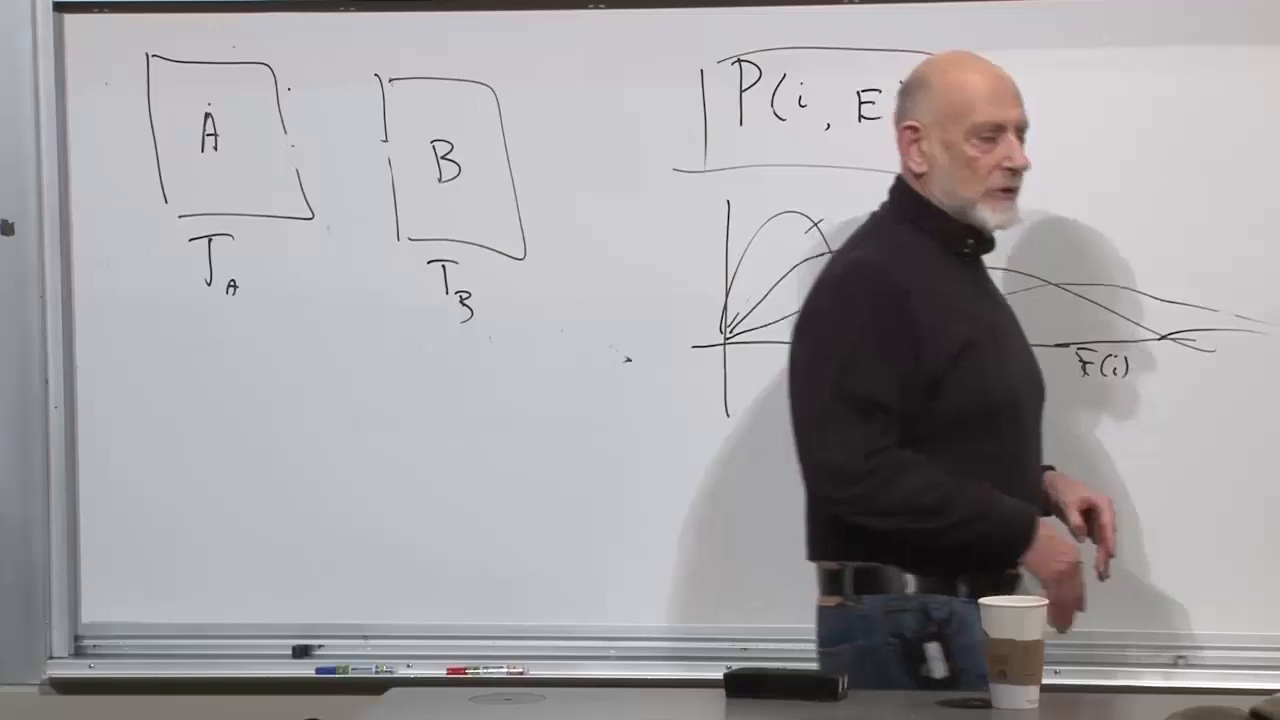
\includegraphics[width=0.88\textwidth]{lecture_02_figure_05.png}
\caption{分别制备的系统\(A\)和\(B\)，以温度\(T_A\)和\(T_B\)标记，就在考虑弱热接触之前。}
\lectureframe{00:48:55}
\end{figure}

\begin{figure}[t]
\centering
\begin{tikzpicture}[>=Stealth]
\draw[rounded corners,thick,fill=blue!6] (0,0) rectangle (2.6,2.4);
\draw[rounded corners,thick,fill=orange!8] (5.4,0) rectangle (8,2.4);
\draw[thick] (2.6,1.35) -- (5.4,1.35);
\draw[thick] (2.6,1.05) -- (5.4,1.05);
\draw[<->,very thick] (3.15,1.2) -- (4.85,1.2)
  node[midway,above] {\(\delta E\)};
\node at (1.3,1.45) {\Large \(A\)};
\node at (6.7,1.45) {\Large \(B\)};
\node at (1.3,0.65) {\(T_A,S_A,E_A\)};
\node at (6.7,0.65) {\(T_B,S_B,E_B\)};
\node at (4,0.35) {\small weak thermal contact};
\end{tikzpicture}
\caption{能量通过弱接触涨落，而组合系统保持隔离。}
\end{figure}

假设，不失一般性，
\begin{equation}
 T_B>T_A.
 \label{eq:sm2-temperature-order}
\end{equation}
经验表明\(B\)应当失去能量，而\(A\)应当获得能量。三个事实将这一预期转化为计算。

\subsection{熵的可加性}

对于两个弱耦合的子系统，其微观选择独立组合，联合可能性的数目相乘：
\[
 W_{AB}=W_AW_B.
\]
熵是对数，因此
\begin{equation}
 S_{\mathrm{tot}}=S_A+S_B.
 \label{eq:sm2-entropy-additivity}
\end{equation}
同样的结果可以直接从乘积分布的香农熵得到。

\begin{classroomqa}
\classquestion{为什么组合系统的熵会相加？}
\lecturerresponse{因为底层可能性的数目相乘，而熵取对数：
\(\log(W_AW_B)=\log W_A+\log W_B\)。弱相互作用正是允许子系统描述和这种领头可加形式的原因。
\lecturetimestamp{00:51:06--00:52:03}}
\end{classroomqa}

\subsection{第一定律和第二定律}

复合系统是孤立的，因此内部交换的能量守恒：
\begin{equation}
 dE_A+dE_B=0,
 \qquad
 dE_B=-dE_A.
 \label{eq:sm2-first-law}
\end{equation}
这就是本实验中的第一定律。

这里把第二定律当作一个公设，稍后再作更深入的说明。
当相连的两个系统向新的平衡态弛豫时，
\begin{equation}
 dS_{\mathrm{tot}}=dS_A+dS_B\geq0.
 \label{eq:sm2-second-law}
\end{equation}
严格不等式描述的是偏离平衡态的自发弛豫；
在平衡态下，对于可逆的一阶变分，等号成立。

最后，温度的定义适用于每个子系统：
\begin{equation}
 dE_A=T_A\,dS_A,
 \qquad
 dE_B=T_B\,dS_B.
 \label{eq:sm2-two-temperatures}
\end{equation}

\begin{figure}[H]
\centering
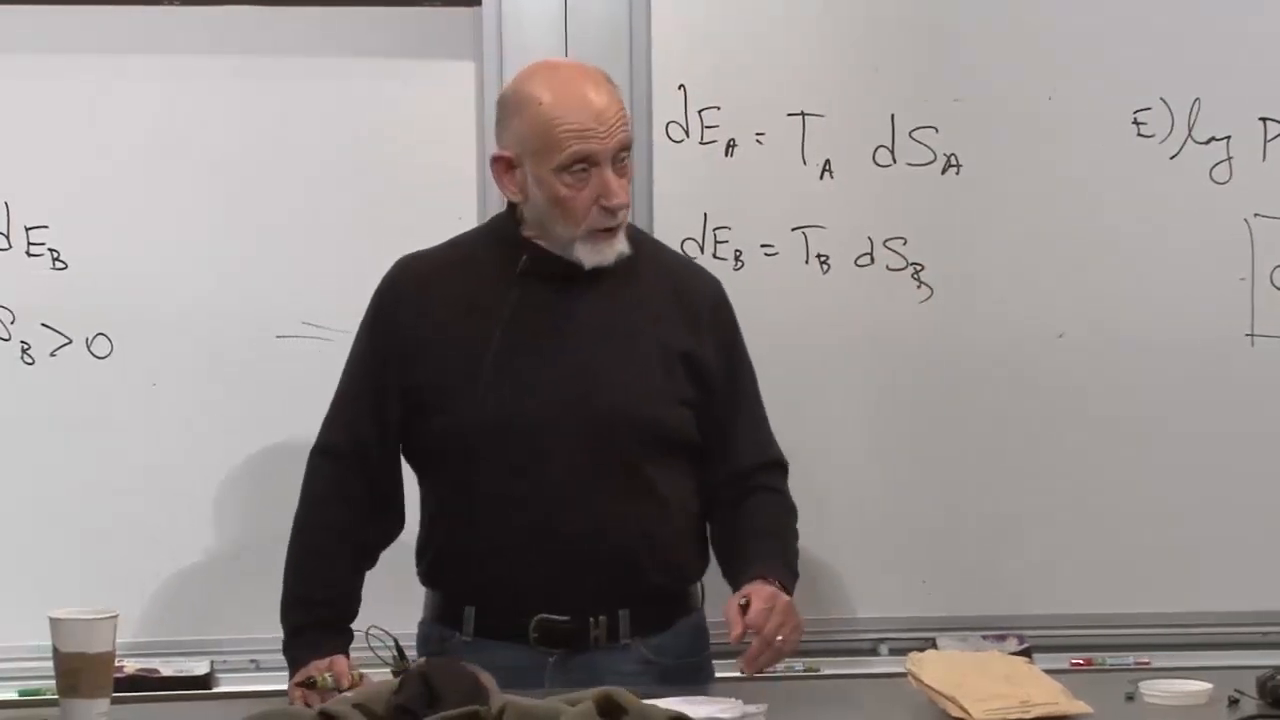
\includegraphics[width=0.88\textwidth]{lecture_02_figure_06.png}
\caption{黑板论证结束时给出的两个子系统关系式
\(dE_A=T_A\,dS_A\) 和 \(dE_B=T_B\,dS_B\)。}
\lectureframe{00:54:00}
\end{figure}

\subsection{能量流动的符号}

这些方程已经确定了净传递的方向。将
\(dS_A=dE_A/T_A\)、\(dS_B=dE_B/T_B\) 和
\eqref{eq:sm2-first-law} 代入 \eqref{eq:sm2-second-law}：
\begin{align}
 dS_{\mathrm{tot}}
 &=\frac{dE_A}{T_A}+\frac{dE_B}{T_B}\\
 &=dE_A\left(\frac{1}{T_A}-\frac{1}{T_B}\right)\geq0.
 \label{eq:sm2-flow-sign}
\end{align}
如果 \(T_B>T_A>0\)，那么
\[
 \frac{1}{T_A}-\frac{1}{T_B}>0.
\]
因此方程 \eqref{eq:sm2-flow-sign} 要求
\[
 dE_A>0,
 \qquad
 dE_B<0.
\]
较冷的系统 \(A\) 获得能量，较热的系统 \(B\) 失去能量。
当 \(T_A=T_B\) 时，一阶熵变不提供任何优先方向，微观交换相互抵消，净流动为零。于是，
抽象的导数 \(T=dE/dS\) 再现了热与冷的操作区分。